\section{Introduction}
\frame{
    {Historique}
    \begin{columns}
        \column{0.5\textwidth}
        \begin{itemize}
            \item Prononciation \og Lah-tec \fg{}
            \item Language et composition de document \\
                Permet de surtout se concentrer sur le fond
            \item Créé par Leslie Lamport (années 1980)
            \item Utilisé principalement dans les domaines académiques et aussi techniques
        \end{itemize}
        \column{0.5\textwidth}
        \centering
        
\includegraphics[width=0.6\textwidth]{LaTeX_logo.png}
        \\
        \vspace{1cm}
        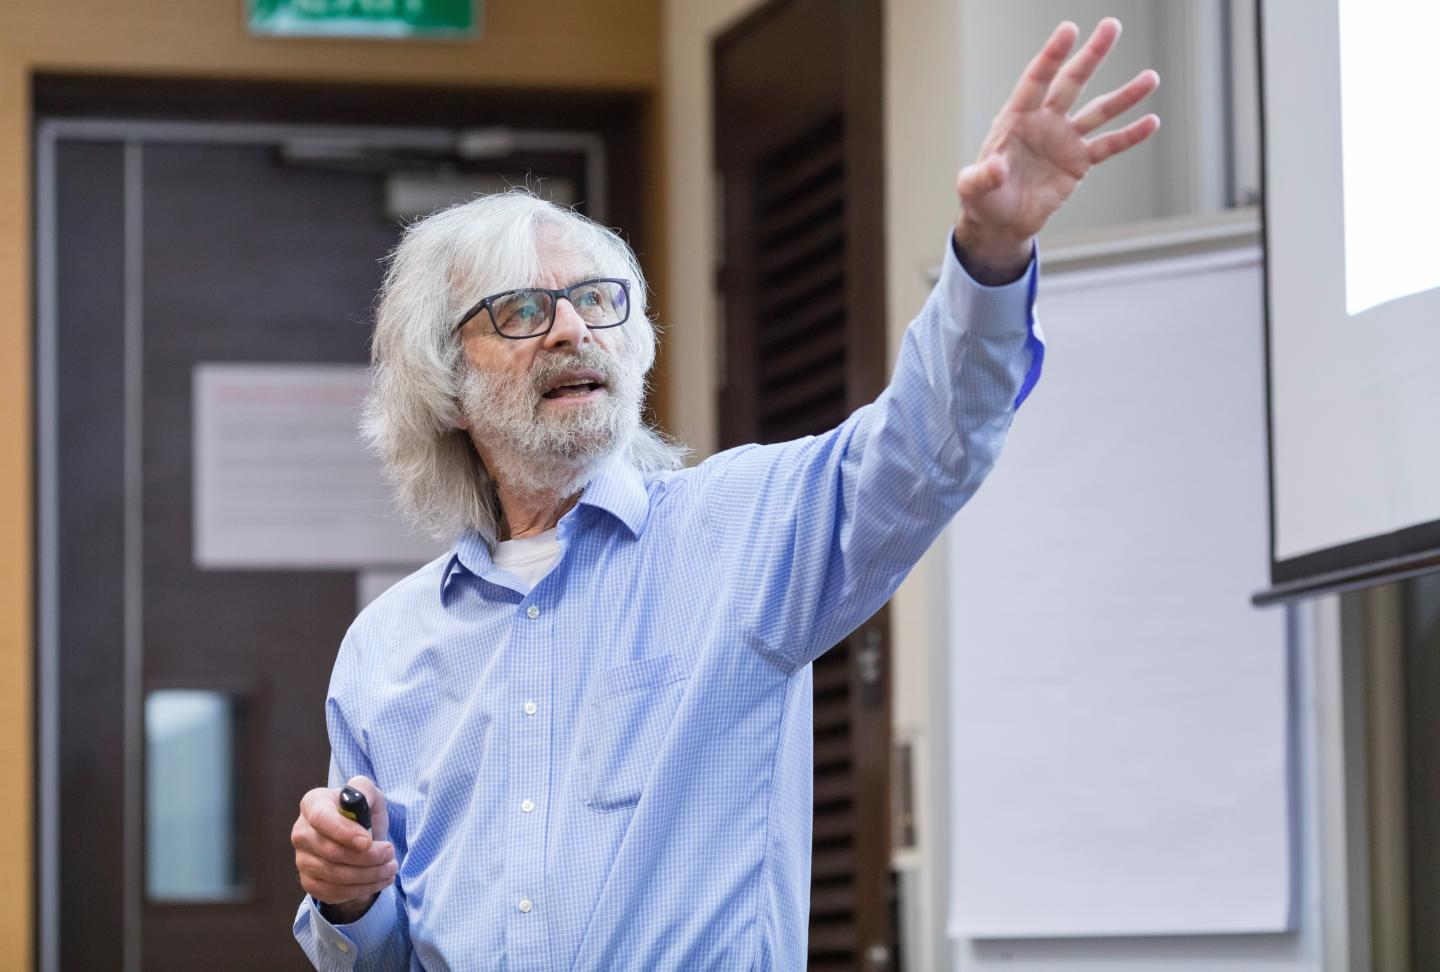
\includegraphics[width=0.6\textwidth]{Leslie_Lamport2.jpg}
    \end{columns}
}

\frame{
    {Principes d'utilisation}
    \begin{itemize}
        \item Langage informatique de balisage (comme HTML)
        \item Utiliser un éditeur de texte (NotePad++; pas MS Word)
        \item Macro-commandes et compilateur sont à utiliser
    \end{itemize}
}
